\documentclass{article}
\usepackage{amsmath}
\usepackage{amsfonts}
\usepackage[english]{babel}
\usepackage[utf8]{inputenc}
\usepackage{amsthm}
\usepackage{graphicx}

\newcommand{\norm}[1]{\left\lVert#1\right\rVert}
\newtheorem{theorem}{Theorem}
\newtheorem{prop}{Proposition}

\begin{document}

\title{HPC hw2}
\author{Toby Harvey}
\maketitle

While I implemented all the GPU functions for find edges, I became particularly  interested in the reductions for min and max. I decided to take two different strategys for the reduction, both share the same basic scheme in which each column of an array is split into a constant number of blocks. I partitioned the array like this because I assumed the GPU will access memory contigiously by column. If we are comparing two elements then the GPU has a chance of reading both at the same time. Once a reduction is done on every single block of the Array we have effectively 1-dimensionalized our Array to vector of block-mins or block-maxs. From there we can again reduce the vector on the GPU with a almost identical algorthim (our indices are just no longer two dimensional). I choose to experiement with how to compare elements/what the stride between elements in a block should be for each comparison by a thread. One way (that jeremy implemented) is shown in my drawing, in which we stride by the number of threads or half the number of elements in a block. Alternatively, I also tried striding just to a neighbor, as shown in the right side of my drawing. My thinking was that the GPU would definitely read both an element and its neighbor at the same time which would improve bandwidth, where as there still my be a chance they arent read together in the larger strided version. The the second two figures compare the speed of each implementation.

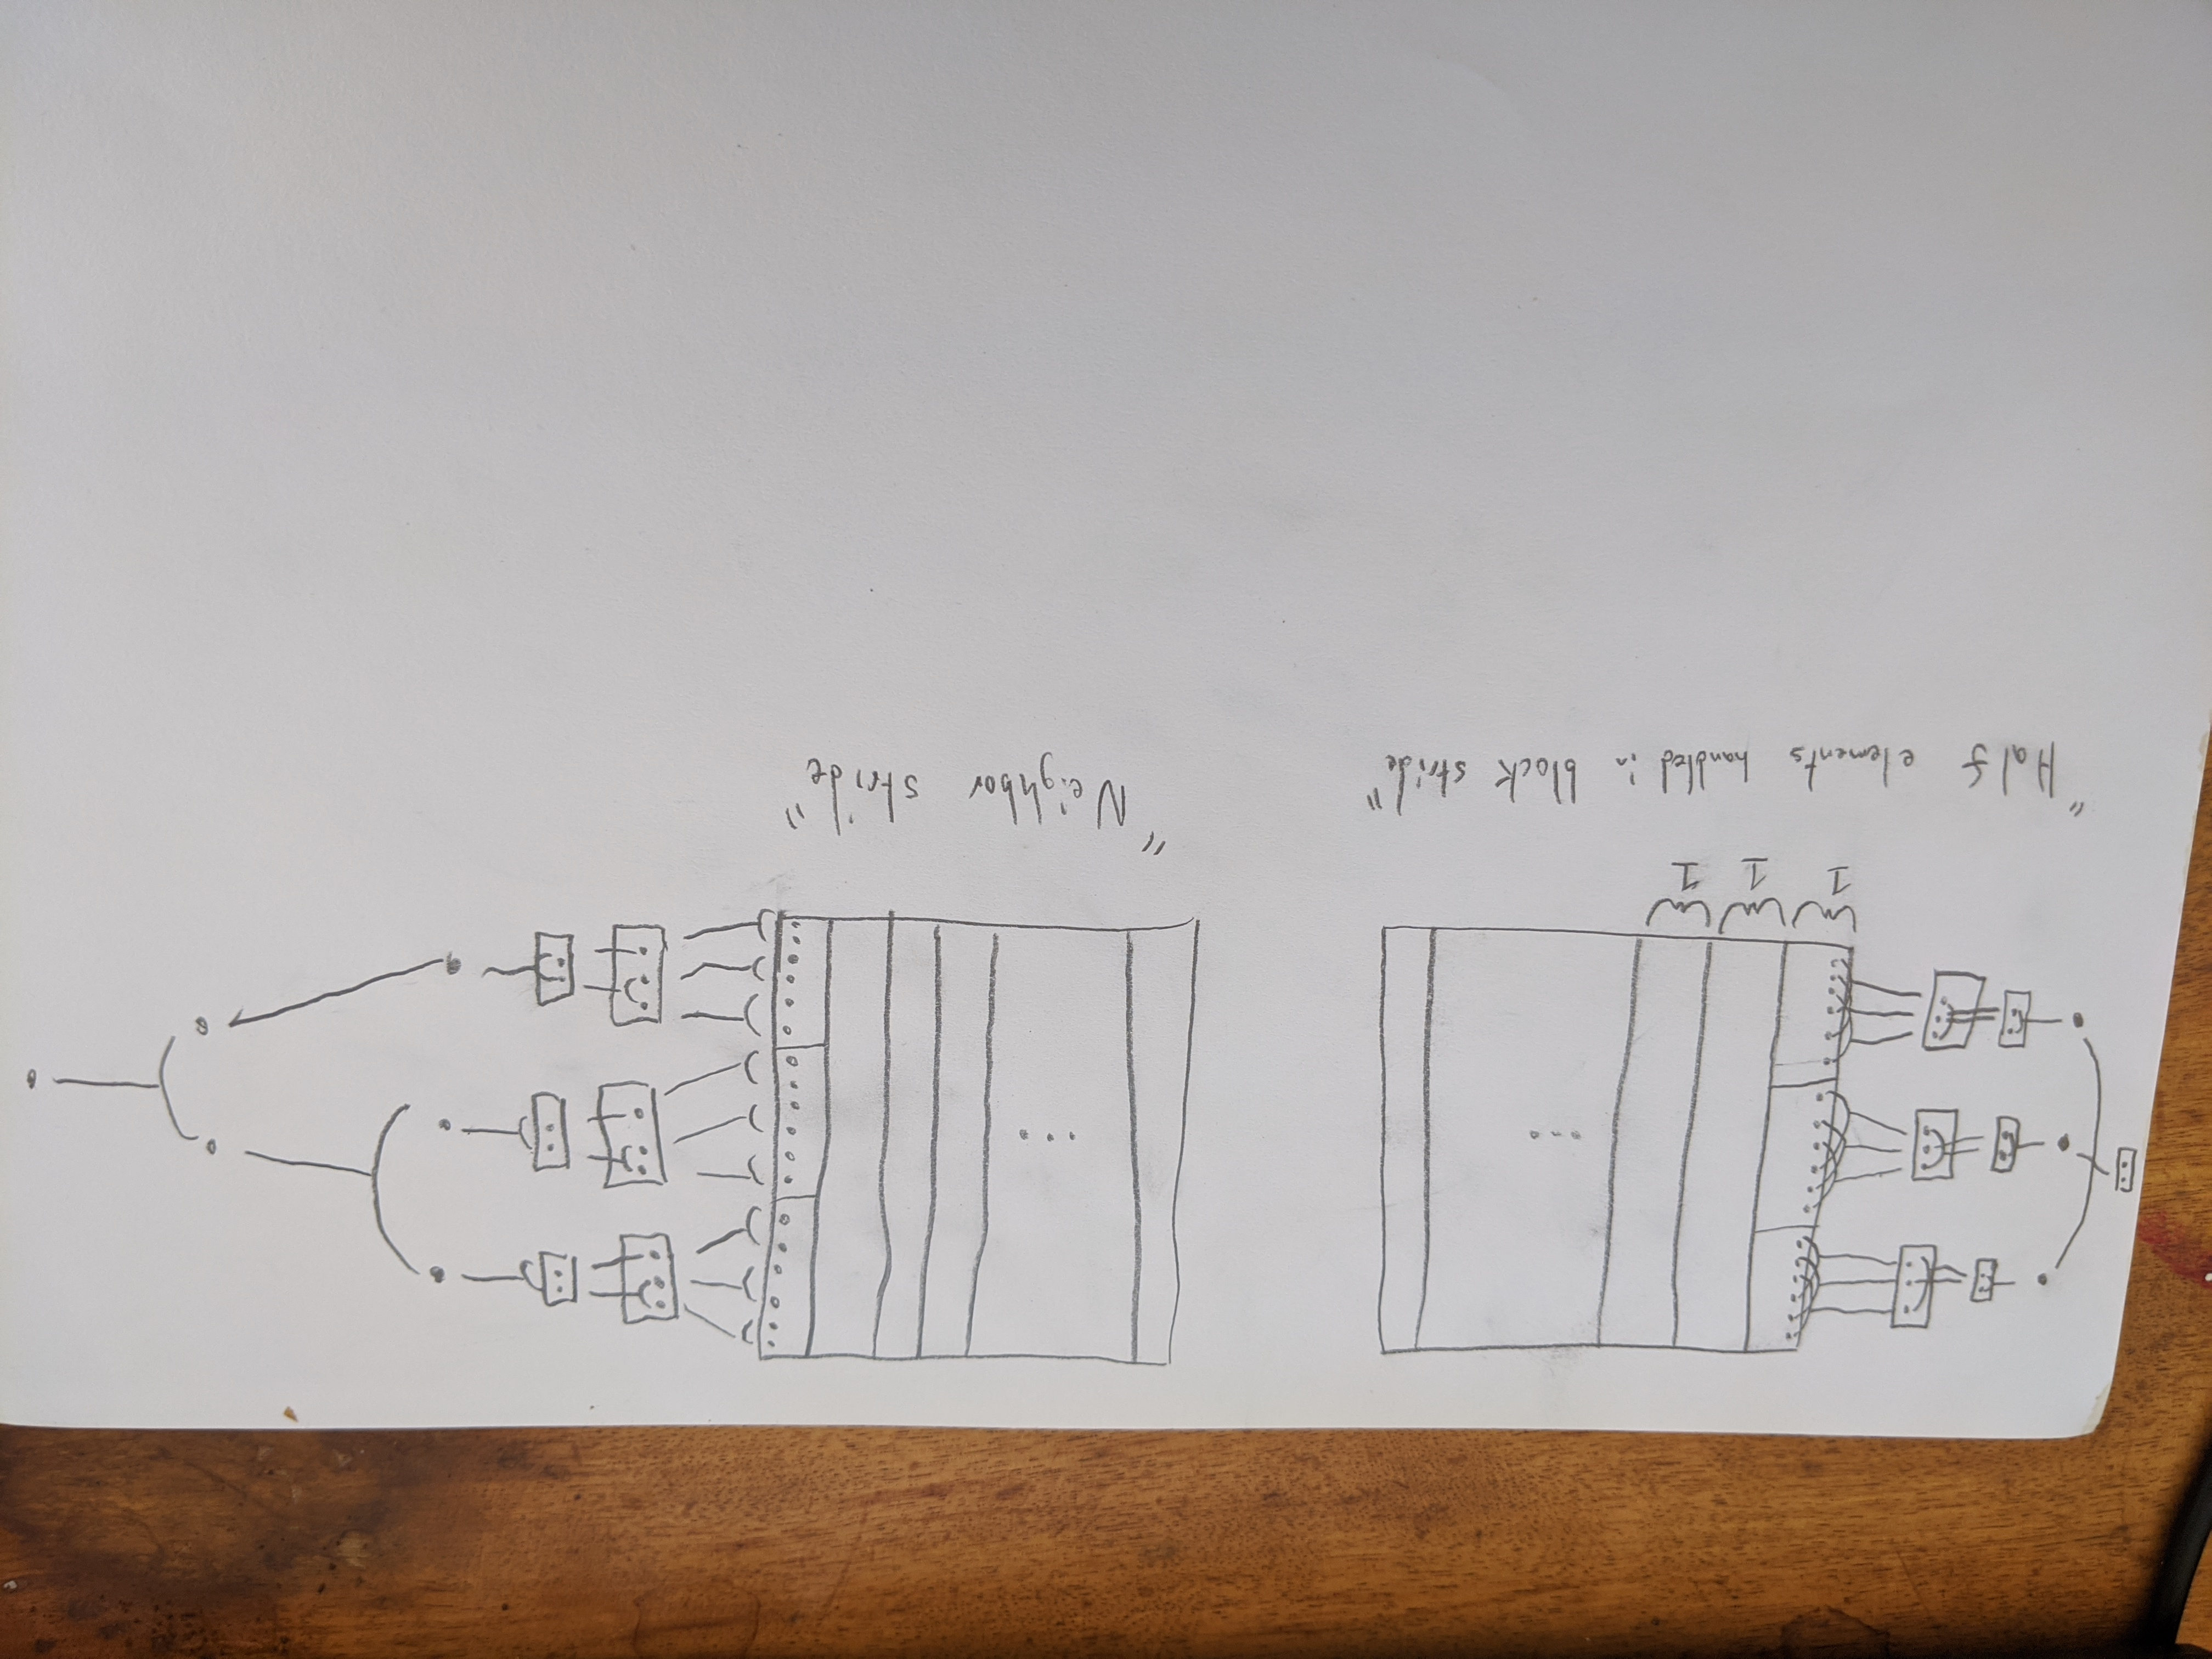
\includegraphics[width=15cm, height=10cm, angle=180]{pic.jpg}
\newpage
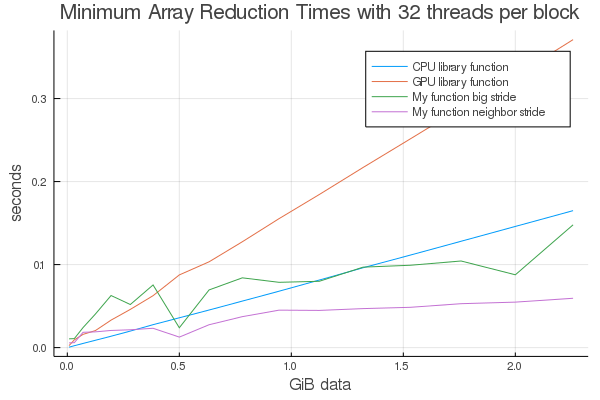
\includegraphics[scale=.5]{stide_comp.png}

\vspace{3mm}

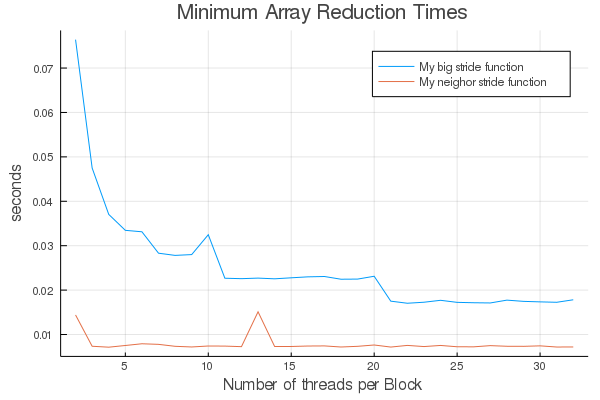
\includegraphics[scale=.5]{thread_comp.png}




\end{document}
